% 
% Permission is granted to copy, distribute and/or modify this document
% under the terms of the GNU Free Documentation License, Version 1.2
% or any later version published by the Free Software Foundation;
% with no Invariant Sections, no Front-Cover Texts, and no Back-Cover
% Texts.  A copy of the license is included in the section entitled "GNU
% Free Documentation License".

\documentclass[11pt]{article}

\usepackage{OTICP_Documentation}
\usepackage{Math_Notations}

\makeindex

\begin{document}

\thispagestyle{empty}

% 
% Permission is granted to copy, distribute and/or modify this document
% under the terms of the GNU Free Documentation License, Version 1.2
% or any later version published by the Free Software Foundation;
% with no Invariant Sections, no Front-Cover Texts, and no Back-Cover
% Texts.  A copy of the license is included in the section entitled "GNU
% Free Documentation License".
\vspace*{2cm}

\begin{center}
  {\huge \bf Documentation of the OTICP module}
  \input{GenericInformation.tex}
\end{center}



\newpage
%  
%  Permission is granted to copy, distribute and/or modify this document
%  under the terms of the GNU Free Documentation License, Version 1.2
%  or any later version published by the Free Software Foundation;
%  with no Invariant Sections, no Front-Cover Texts, and no Back-Cover
%  Texts.  A copy of the license is included in the section entitled "GNU
%  Free Documentation License".
\vspace{0.5in}
\begin{center}
\vspace{0.3in}
\emph{\fontshape{sc} Abstract}
\vspace{0.5in}
\end{center}

The purpose of this document is to present the OTICP module.

This document is organized according to the OpenTURNS documentation :
\begin{itemize}
\item a \itshape{Reference Guide} which gives some theoretical basis,
\item a \itshape{Use cases Guide} which details scripts in python (the Textual Interface language of OpenTURNS) and helps the User to learn as quickly as possible the manipulation of the $integralcompoundpoisson$ module,
\item the \itshape{User Manual} which details the $integralcompoundpoisson$ objects and give the list of their methods,
\item the \itshape{Examples Guide} which provides example scripts performed with the $integralcompoundpoisson$ module.
\end{itemize}


\tableofcontents
\newpage
% 
% Permission is granted to copy, distribute and/or modify this document
% under the terms of the GNU Free Documentation License, Version 1.2
% or any later version published by the Free Software Foundation;
% with no Invariant Sections, no Front-Cover Texts, and no Back-Cover
% Texts.  A copy of the license is included in the section entitled "GNU
% Free Documentation License".




%%%%%%%%%%%%%%%%%%%%%%%%%%%%%%%%%%%%%%%%%%%%%%%%%%%%%%%%%%%%%%%%%%%%%%%%%%%%%%%%%%%%%%%%%% 
\section{Reference Guide}

\subsection{Definition}

In probability theory, a \emph{compound Poisson distribution}  is the sum of a Poisson-distributed number of independent identically-distributed random variables. In the simplest cases, the result can be either a continuous or a discrete distribution.\\
If $N$ is a poisson distributed variable and if $(X_i)_i$ are identically distributed random variables that are mutually independent and also independent of $N$, then :

\begin{equation}
Y = \left( \displaystyle \sum_{i=1}^{N}X_i \right)\fcar{N\geq 1}
\end{equation}

is a compound Poisson distribution.\\

This module only focuses on  variables $X_i$ which are discrete, with finite range and integer values. We name this particular case the \emph{Integral Compound Poisson Distribution}. It implies that the compound Poisson distribution is also discrete, with finite range and integer values. Then, it allows the use of its generating function in order to evaluate its probability distribution.




\subsection{Distribution of the Integral Compound Poisson Distribution }\label{loiY}

Let us suppose that the variables $(X_i)_i$ are identically and independently distributed according to the $X$ distribution and that $N$ follows a Poisson distribution parameterised by $\lambda$.\\

The generating function of $N$ is, for $z\in[-1, 1]$ :
\begin{eqnarray}\label{PhiN}
\phi_{N}(z) = E[z^{N}] = e^{-\lambda(1-z)}
\end{eqnarray}

We show that the generating function of $Y$ writes :
\begin{eqnarray}
\phi_{Y}(z) = \phi_{N} \circ \phi_{X}(z)
\end{eqnarray}

Then, the probability distribution of $Y$ is derived from its generating function as follows :
\begin{eqnarray}
\forall n \in \mathbb{N}, \, \, \mathbb{P}(Y = n) = \displaystyle \left. \frac{1}{n!}\frac{d^{(n)}\phi_{Y}(z)}{dz^n } \right|_{z=0}
\end{eqnarray}


%%%%%%%%%%%%%%%%%%%%%%%%%%%%%%%%%%%%%%%%%%%%%%%%%%%%%%
\subsection{Algorithmic details}

The evaluation of the integral compound Poisson distribution is based on the previous results. The references \cite{Abate}, \cite{Stoer} and \cite{Feller} give more details on these results. We develop below some important points : the Cauchy's integral formula and the Poisson summation formula.

\subsubsection{Cauchy's integral formula}

In mathematics, Cauchy's integral formula, named after Augustin-Louis Cauchy, is a central statement in complex analysis. It expresses the fact that a holomorphic function defined on a disk is completely determined by its values on the boundary of the disk, and it provides integral formulas for all derivatives of a holomorphic function. Cauchy's celebrated formula shows that, in complex analysis, differentiation is equivalent to integration.\\

{\bf Cauchy Formula :} Suppose $U$ is an open subset of the complex plane $C$, $f : U \rightarrow C$ is a holomorphic function and the closed disk $D = \{ z : | z - z_0| = r\}$ is completely contained in $U$. Let $\gamma$ be the circle forming the boundary of $D$. Then for every a in the interior of $D$:

Let $f$ be a a holomorphic function on $\mathcal{U}$  an open subset of the complex plane $\mathbb{C}$, $K$ a compact of $\mathcal{U}$ completely contained in $\mathcal{U}$ and $\Gamma$ its boundary. Then for every $z_0 \in K-\Gamma$, we have : 
\begin{eqnarray}\label{forCauchy}
 f(z_0).1_{\Gamma}(z_0)= \displaystyle \frac{1}{2i\pi}\int_{\Gamma} \frac{f(u)}{u-z_0}du
\end{eqnarray}
where $1_{\Gamma}(z_0) = \int_{\Gamma} \frac{1}{u-z_0}du$.\\

With $\Gamma = Circle(0,r)$ and $z_0 = 0$, then the relation  (\ref{forCauchy}) writes : 
\begin{eqnarray}\label{f20}
f(0) = \displaystyle \frac{1}{2i\pi}\int_{\Gamma} \frac{f(u)}{u}du
\end{eqnarray}
and we show that : 
\begin{eqnarray}\label{fn20}
f^n(0) = \displaystyle \frac{n!}{2i\pi}\int_{\Gamma} \frac{f(u)}{u^{n+1}}du
\end{eqnarray}

Then, with a proper parametrisation of the circle, we have: 
\begin{eqnarray}\label{fn20Pol}
f^n(0) = \displaystyle \frac{n!}{2\pi r^n}\int_{0}^{2\pi} f\left(re^{i\theta}\right)e^{-in\theta} d\theta
\end{eqnarray}


The relation (\ref{fn20Pol}) applied to the generating function $\phi$ of $Y$ writes :
\begin{eqnarray}\label{pnCauchy}
p_n = \displaystyle \frac{1}{2\pi r^n}\int_{0}^{2\pi} \phi\left(re^{i\theta}\right)e^{-in\theta} d\theta
\end{eqnarray}



\subsubsection{Poisson summation formula}

In mathematics, the Poisson summation formula is an equation that allows us to relate the Fourier series coefficients of the periodic summation of a function to values of the function's continuous Fourier transform. Consequently, the periodic summation of a function is completely defined by discrete samples of the original function's Fourier transform. And conversely, the periodic summation of a function's Fourier transform is completely defined by discrete samples of the original function. The Poisson summation formula was discovered by Siméon Denis Poisson and is sometimes called Poisson resummation.\\

The relation (\ref{pnCauchy}) requires the Poisson summation formula.\\

Let  $g$ be a function from $\mathbb{R}$ into $\mathbb{R}$ as:
\begin{eqnarray}\label{g2u}
g(u) = \sum_{k=-\infty}^{+\infty} a_k e^{iku}
\end{eqnarray}
then $a_n$ writes :
\begin{eqnarray}\label{an}
a_n = \frac{1}{2\pi}\int_{0}^{2\pi} g(u)e^{-in\theta} d\theta
\end{eqnarray}
If we consider the periodic suite :
\begin{eqnarray}\label{anp}
a_n^p =  \sum_{k=-\infty}^{+\infty} a_{n+km}
\end{eqnarray}
for a given integer $m$, we show that $a_n^p$ can write as : 
\begin{eqnarray}\label{anp2}
a_n^p =  \displaystyle \frac{1}{m} \sum_{k=0}^{m-1} g\left(\frac{2\pi k}{m}\right)e^{-\frac{2i\pi kn}{m}}
\end{eqnarray}
whioch leads to the  {\bf Poisson summation formula :}
\begin{eqnarray}\label{forSomPoisson}
\sum_{k=0}^{m-1} g\left(\frac{2\pi k}{m}\right)e^{-\frac{2i\pi kn}{m}} = m \sum_{k=-\infty}^{+\infty}a_{n+km}
\end{eqnarray}

The figure \ref{FigAnp} gives an illustration of the periodic suite $a_n$.

\begin{figure}[Hhbtp]
     \begin{center}
      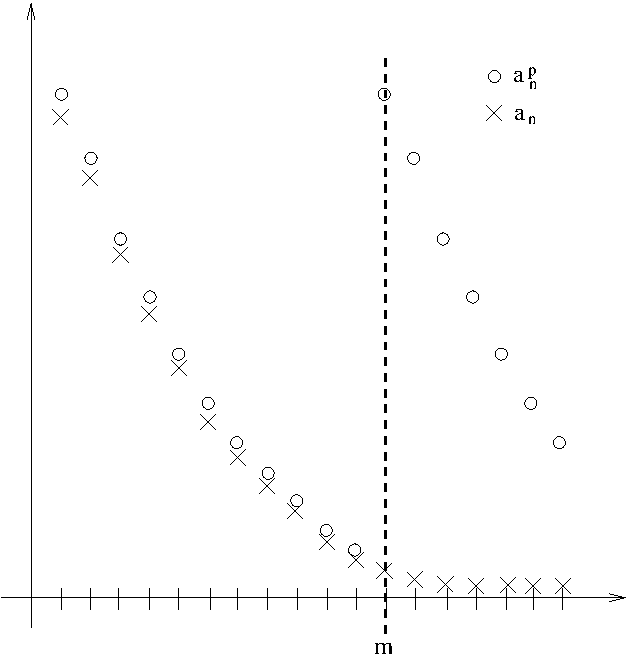
\includegraphics[width=8cm]{figAnp.pdf} 
      \caption{Periodic suite $a_n$.}
      \label{FigAnp}
    \end{center}
 \end{figure}





As the function $g$ writes as a convergent serie (\ref{g2u}), $|a_k| \underset{k \rightarrow +\infty}{\rightarrow} 0$. Then if we take $m$ great enough, we obtain the following approximation : 
\begin{eqnarray}\label{anpApprox}
a_n^p  =  \sum_{k=-\infty}^{+\infty} a_{n+km} \simeq a_n
\end{eqnarray}

In our probabilistic context, the function $g$ is : 
\begin{eqnarray}\label{cadreProb}
g(u) = \phi\left(re^{iu}\right) = \sum_{k=0}^{+\infty}p_k r^k e^{iku}
\end{eqnarray}
wich leads to the expression (\ref{g2u}) with
\begin{equation}\label{cadreProb2}
\left\{
\begin{array}{ll}
  a_k = 0, & \forall k<0 \\
  a_k = p_kr^k & \forall k \geq 0
\end{array}
\right.
\end{equation}

The relation (\ref{forSomPoisson}) writes, for $n < m$ and for the function $g$ defined in (\ref{cadreProb2})  :
\begin{eqnarray}\label{forSomPoissonG}
m \sum_{k=0}^{+\infty}a_{n+km} = \sum_{k=0}^{m-1} g\left(\frac{2\pi k}{m}\right)e^{-\frac{2i\pi kn}{m}}
\end{eqnarray}
By isolating the term $a_n$ in (\ref{forSomPoissonG}), we have : 
\begin{eqnarray}\label{termeAn}
a_n = \displaystyle \frac{1}{m} \sum_{k=0}^{m-1} g\left(\frac{2\pi k}{m}\right)e^{-\frac{2i\pi kn}{m}} - \sum_{k=1}^{+\infty}a_{n+km}
\end{eqnarray}
which, within the probabilistic context of (\ref{cadreProb}) and (\ref{cadreProb2}) leads to the expression of $p_n$ : 
\begin{eqnarray}\label{pnApprox}
p_n = \displaystyle \frac{1}{mr^n} \sum_{k=0}^{m-1} \phi\left(re^{\frac{2i\pi k}{m}}\right) e^{-\frac{2i\pi kn}{m}} - e_d
\end{eqnarray}
where $e_d$ is the approximation error done if we neglige this term in (\ref{pnApprox}). This error writes : 
\begin{eqnarray}\label{ed}
e_d = \displaystyle \sum_{k=1}^{+\infty}p_{n+km}r^{km}
\end{eqnarray}
and can be bounded, for $0 < r < 1$ : 
\begin{eqnarray}\label{edEncadr}
0 < e_d \leq  \sum_{k=1}^{+\infty}r^{km} = \displaystyle \frac{r^m}{1-r^m}
\end{eqnarray}
Thus, the precision of the evaluation of $p_n$ is given by the choice of the couple $(m,r)$.\\

We have the following final result : 
\begin{eqnarray}\label{pnApprox2}
\forall n < m, \, \, p_n \simeq \hat{p}_n = \displaystyle \frac{1}{mr^n} \sum_{k=0}^{m-1} \phi\left(re^{\frac{2i\pi k}{m}}\right) e^{-\frac{2i\pi kn}{m}}
\end{eqnarray}
where
\begin{eqnarray}\label{erreurRel}
\displaystyle |p_n - \hat{p}_n | \leq  \frac{r^m}{1-r^m}
\end{eqnarray}


\subsubsection{Fast Fourier Transform (FFT)}

In order to optimize the numerical evaluation of the $(\hat{p}_n)_n$ given in (\ref{pnApprox2}), it is recommended to use the Fast Fourier Transform (FFT) which evaluates simultaneously the values $(p_0, \hdots, p_{m-1})$ with an optimised cost.\\

The relation (\ref{pnApprox2}) presents $mr^np_n$ as the result of a discrete Fast Fourier Transform of the suite $\left(\phi\left(re^{\frac{2i\pi k}{m}}\right)\right)_{k \geq 0}$.\\
If we chose $m$ as a power of 2, we can evaluate $(p_0, \hdots, p_{m-1})$ thanks to the FFT. The algorithmic cost is no more $\mathcal{O}(m^2)$ but  $\mathcal{O}(m\log m)$.





%\subsection{References}


\addcontentsline{toc}{subsection}{Bibliographie}
\begin{thebibliography}{9}
  \bibitem {Abate} J. Abate, W. Whitt,
     \emph{The Fourier-series method for inverting transforms of probability distributions.}
     Queueing Systems, feb. 1991.
  \bibitem {Stoer}J. Stoer, R. Bulirsch,
     \emph{Introduction to numerical analysis.}
     Springer, Third Edition, 2002.
  \bibitem {Feller} W. Feller,
     \emph{Introduction to probability theory and its application.}
     Wiley, Second Edition, vol 2, 1971.
\end{thebibliography}




\newpage
% 
% Permission is granted to copy, distribute and/or modify this document
% under the terms of the GNU Free Documentation License, Version 1.2
% or any later version published by the Free Software Foundation;
% with no Invariant Sections, no Front-Cover Texts, and no Back-Cover
% Texts.  A copy of the license is included in the section entitled "GNU
% Free Documentation License".




%%%%%%%%%%%%%%%%%%%%%%%%%%%%%%%%%%%%%%%%%%%%%%%%%%%%%%%%%%%%%%%%%%%%%%%%%%%%%%%%%%%%%%%%%% 
\section{Use Cases Guide}


\subsection{UC1 : Creation and manipulation of an {\itshape IntegralUserDefined} variable}

This Use Case explicitates how to create and manipulate an $IntegralUserDefined$ variable which is a discrete variable with finite range and integer values.
\espace



\requirements{
  \begin{description}
  \item[$\bullet$] values of the range and associated probabilities : $range$ and $weights$
  \item[type:]  $range$ a python list of integers, $weights$ a list of reals, with unit sum or not
  \item[$\bullet$] or $sample$ a numerical sample of the discrete variable $X$
  \item[type:] a $NumericalSample$
  \end{description}
}
{
  \begin{description}
  \item[$\bullet$] a discrete variable with finite range and integer values : {\itshape myX}
  \item[type:] IntegralUserDefined
  \end{description}
}


\espace
Python  script for this Use Case :
\begin{lstlisting}

##############################################################################
# CASE 1 : Creation from the range values and the associated probabilities
##############################################################################

# Creation of the python list of the range (integers only)
# for example : 5, 7, 32
range = [5,7,32]

# Creation of the associated probabilities list
poidweightss = [0.1, 0.2, 0.3, 0.4]

# Creation of the IntegralUserDefined variable
myX = IntegralUserDefined(range, weights)

# Other signature
myX = IntegralUserDefined(UnsignedIntegerCollection(range), ...
     ... NumericalPoint(weights))


#########################################################
# CASE 2 : Creation form a numerical sample
#########################################################

# Creation of the IntegralUserDefined variable
myX = IntegralUserDefinedFactory.buildImplementation(sample)


########################################
# Manipulation of the IntegralUserDefined
########################################

# Get the range
print "range=", myd_Sc.getRange()

# Get thes weights 
print "weights=", myX.getWeights()

# Generate a realisation
print "realization=", myX.getRealization()

# Generate a numerical samplee
size = 10
print "numerical sample=", myX.getNumericalSample(size)

# Compute the probability of a particular state
print "weight of the value ", 5, "=", myX.computePDF(5)

# Compute the CDF of a particular state 
print "CDF at ", 5, "=", myX.computeCDF(5)
\end{lstlisting}




%%%%%%%%%%%%%%%%%%%%%%%%%%%%%%%%%%%%%%%%%%%%%%%%%%%%%%%%%%%%%%%%%%%%%%%%%%%%%%%%%
\subsection{UC2 : Creation and manipulation of an  {\itshape IntegralCompoundPoisson} variable}



This Use Case shows how to create and manipulate an {\itshape IntegralCompoundPoisson} variable, defined as :
\begin{equation}
Y = \left( \displaystyle \sum_{i=1}^{N}X_i \right)\fcar{N\geq 1}
\end{equation}

where $N$ is a Poisson distributed variable  parameterised by $\theta > 0$ and $(X_i)_i$  identically distributed random variables, with finite range and integer values. They are also mutually independent and also independent of $N$.

When a variable $Y$ of type $IntegralCompoundPoisson$ is created, all the values $p_k = \mathcal{P}(Y=k)$ are authomatically evaluated for $k \in [0, m-1]$ with $m = 2^{param}$. If the User asks for the evaluation of $p_n$ for $n \geq m$, then Open TURNS authomatically re-evaluates  all the values   $p_k$ for $k \in [0, N]$  with $N   = 2^{E[log_2 n]+1}$ (ie the first power of 2 which is strictly  $>n$).\\

The figures Fig. \ref{ICP_PDF} et Fig.\ref{ICP_CDF} draw the probability distribution and its cumulated probability distribution of an intergal compound distribution defined by : 
\begin{itemize}
  \item $(X_i)_i$ are distributed according to  the discrete distribution of range $[1, 2, 4, 7]$ associated to the respective probabilities $[0.1, 0.2, 0.3, 0.4]$,
  \item $N$ is a Poisson distribution which parameter is $\theta = 20$.
\end{itemize}


\begin{figure}[Hhbtp]
  \begin{minipage}{8cm}
    \begin{center}
      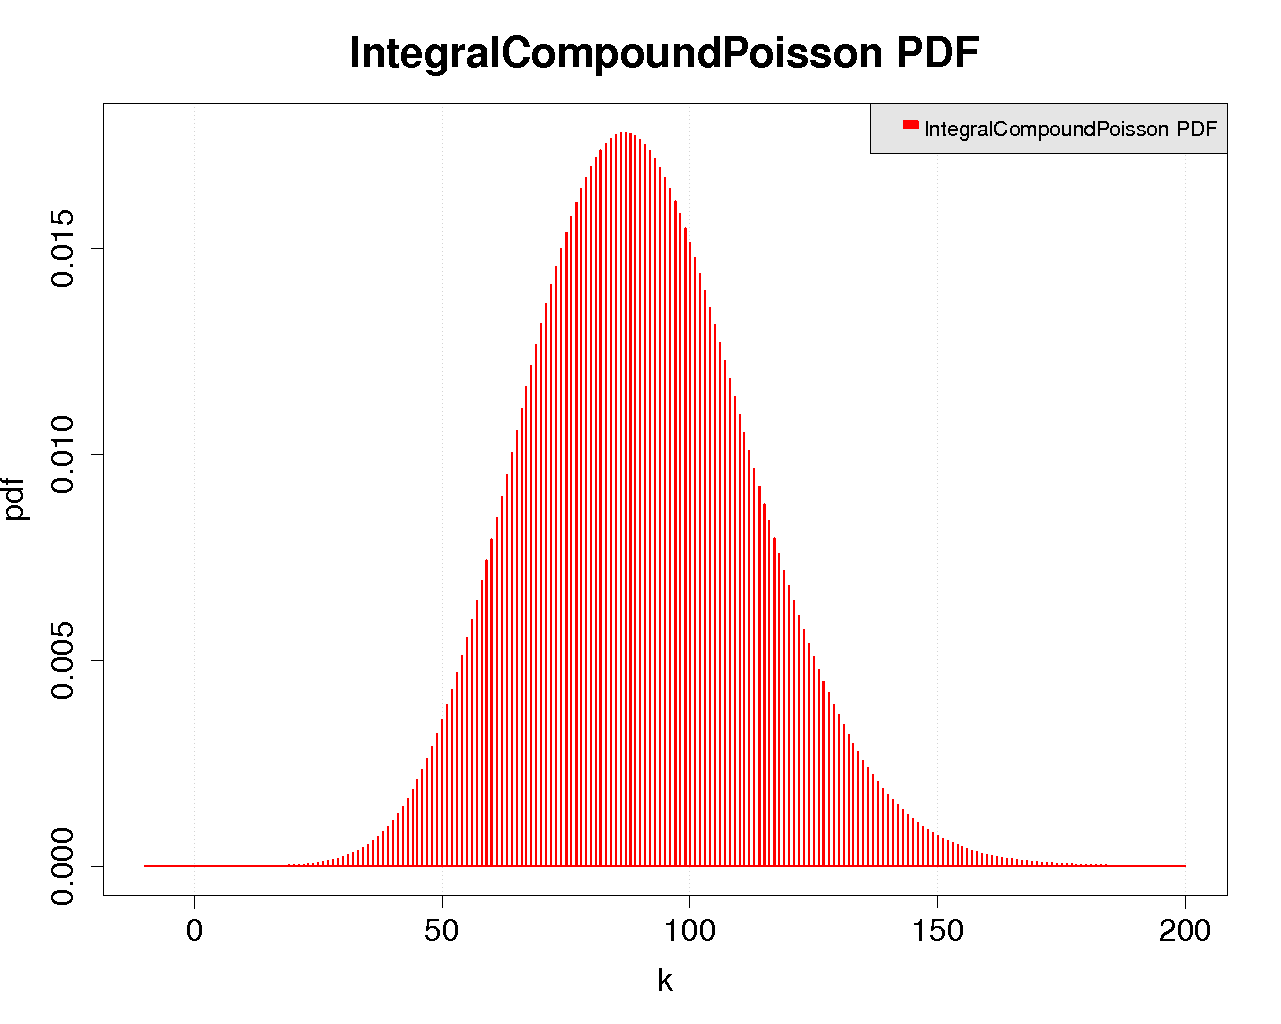
\includegraphics[width=8cm]{ICP_PDF.png} 
      \caption{Probability Distribution of an Integral Compound Poisson distribution.}
      \label{ICP_PDF}
    \end{center}
  \end{minipage}
  \hfill
  \begin{minipage}{8cm}
    \begin{center}
      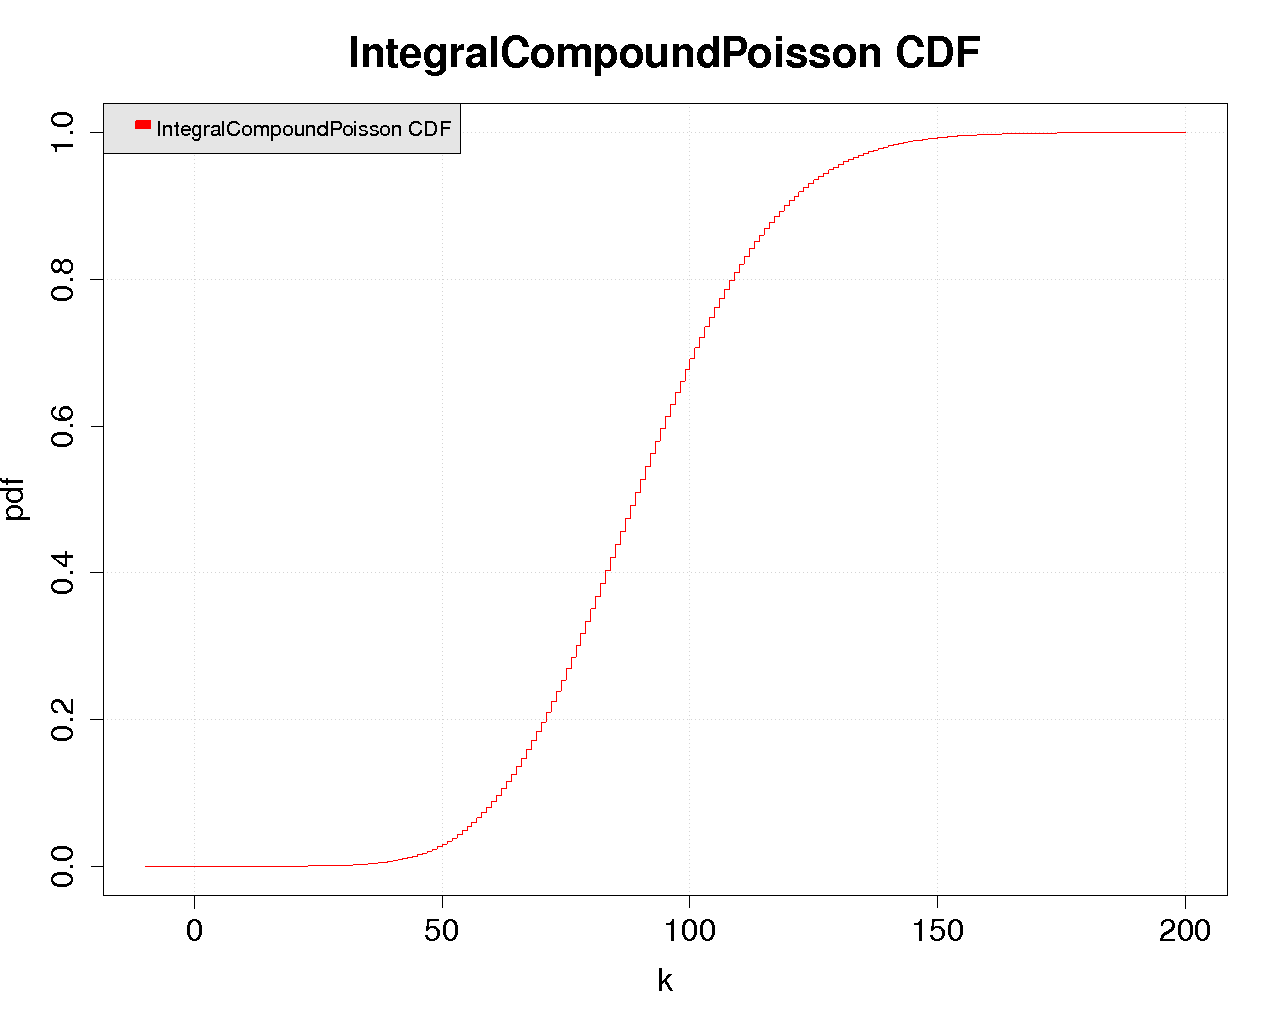
\includegraphics[width=8cm]{ICP_CDF.png} 
      \caption{Cumulated Probability Distribution of an Integral Compound Poisson distribution.}
      \label{ICP_CDF}
    \end{center}
  \end{minipage}
\end{figure}






\espace

\requirements{
 
  \begin{description}
  \item[$\bullet$] a discrete variable with finite range and integer values : {\itshape myX}
  \item[type:] a $IntegralUserDefined$
  \item[$\bullet$] the parameter of the Poisson distribution : {\itshape myTheta}
  \item[type:] a strictly positive real
  \end{description}
}
{
  \begin{description}
  \item[$\bullet$] a Integral Compound Poisson variable  : {\itshape myY}
  \item[type:] a $IntegralCompoundPoisson$
  \end{description}
}

\espace
Python  script for this UseCase :

\begin{lstlisting}
##########################################
# Creation  of the IntegralCompoundPoisson
##########################################

# Creation of the  IntegralCompoundPoisson variable
myY = IntegralCompoundPoisson(myX, myTheta)


###############################################
# Manipulation  of the  IntegralCompoundPoisson
###############################################

# Get the finite discrete distribution myX of type IntegralUserDefined
print "Inside IntegralUserDefined=", myYc.getAtomDistributionD()

# Get the Poisson parameter
print " Poisson parameter=", myY.getTheta()

# Get the param m
print "parameter m=", myY.getM()

# Get the param parameter
print "parameter param=", myY.getLog2cache()

# Generate a realisation of the distribution
print "realisation=", myY.getRealization()

# Compute the PDF at one particular point of the range
print "PDF at ", point, "=", myY.computePCDF(point5)

# Compute the CDF at one particular point of the range
print "CDF at ", point, "=", myY.computeCDF(point5)

# Compute the mean value
print "mean value=", myY.getMean()

# Compute the variance
print "variance=", myY.getCovariance()

# Compute the standard deviation
print "standard deviation=", myY.getStandardDeviation()

# Compute the quantile of order q
print "quantile order", q, "=", myY.computeQuantile(q)
\end{lstlisting}



%%%%%%%%%%%%%%%%%%%%%%%%%%%%%%%%%%%%%%%%%%%%%%%%%%%%%%%%%%%%%%
\subsection{Which python modules to import ?}

In order to use the functionalities described in this documentation, it is necessary to import  : 
\begin{itemize}
   \item the $oticp$ module which uses the $openturns$ module.
\end{itemize}

Python script for this use case :

\begin{lstlisting}
from openturns import *
from oticp import *
\end{lstlisting}

\newpage
% 
% Permission is granted to copy, distribute and/or modify this document
% under the terms of the GNU Free Documentation License, Version 1.2
% or any later version published by the Free Software Foundation;
% with no Invariant Sections, no Front-Cover Texts, and no Back-Cover
% Texts.  A copy of the license is included in the section entitled "GNU
% Free Documentation License".

%%%%%%%%%%%%%%%%%%%%%%%%%%%%%%%%%%%%%%%%%%%%%%%%%%%%%%%%%%%%%%%%%%%%%%%%%%%%%%%%%%%%%%%%%% 
\section{User Manual}

This document gives details on the new methods proposed by the python scripts. 



\subsection{Scripts required}

We describe here the python scripts required by the module : 
\begin{itemize}
  \item $IntegralUserDefined.py$, which implements the IntegralUserDefined class. This class is the UserDefined already contained in Open TURNS, specialised for integral variables.
  \item $IntegralUserDefinedFactory.py$, which gives the functionnalities to adjust a IntegralUserDefined variable to a set of data.
  \item $IntegralCompoundPoisson.py$ which implements the integral compound Poisson distribution.
  \item $Polynomial.py$ which gives functionnalities to manipulate sparse polynomials.
  \item $t\_IntegralUserDefined\_std.py$ which is the test file associated to the IntegralUserDefined class.
  \item $t\_IntegralUserDefinedFactory\_std.py$ which is the test file associated to the IntegralUserDefinedFactory class.
  \item $t\_IntegralCompoundPoisson\_validation.py$ which is the test file associated to the OTICP class.
\end{itemize}


\subsection{IntegralUserDefined}

\begin{description}

\item[Usage :] $IntegralUserDefined(range, weight)$

\item[Arguments :]  \strut
  \begin{description}
  \item $range$ : python list of integers or integer collection of type $UnsignedIntegerCollection$. For example, $range = [5,7,32]$ or $range = UnsignedIntegerCollection([5,7,32])$
  \item $weight$ :  python list of the associated weights or a $NumericalPoint$. If the weights are not normalised, they are authomatically normalised by Open TURNS. For example, $weight = [0.1, 0.2, 0.3, 0.4]$ or  $weight = NumericalPoint([0.1, 0.2, 0.3, 0.4])$.
  \end{description}

\item[Value :] a $IntegralUserDefined$, which is a variable which range ($range$) is  finite with integer values, associated to the weights given in $weight$.

\item[Some methods :]  \strut
  \begin{description}

  \item $getRange$
    \begin{description}
    \item[Usage :] $getRange()$
    \item[Arguments :] none
    \item[Value :]  a $UnsignedIntegerCollection$, which is a python list of integers which are the positive integer values of the range.
    \end{description}
    \bigskip


  \item $getWeights$
    \begin{description}
    \item[Usage :] $getWeights()$
    \item[Arguments :] none
    \item[Value :]  a $NumericalPoint$, the python list of the associated weights. 
    \end{description}
    \bigskip



  \item $getNormalizedWeights$
    \begin{description}
    \item[Usage :] $getNormalizedWeights()$
    \item[Arguments :] none
    \item[Value :]  a $NumericalPoint$, the python list of the associated normalised weights.
    \end{description}

    \end{description}
 
\end{description}





%%%%%%%%%%%%%%%%%%%%%%%%%%%%%%%%%%%%%%%%%%
\subsection{IntegralUserDefinedFactory}


\begin{description}

\item[Usage :] $IntegralUserDefinedFactory$ is a static class which is  used through its unique method $buildImplementation$.

\item[One method :]  $buildImplementation$
    \begin{description}

    \item[Usage :] $buildImplementation(echantillon)$

    \item[Arguments :]  $sample$ : un $NumericalSample$ which represents a numerical sample of the random variable. Its values must be integers.

    \item[Value :]  a $IntegralUserDefined$, a random variable which range is defined by the values f the $sample$. The probability of $k$ is estimated by  $ p_k = \displaystyle \frac{N_k}{n}$ where  $n$  is the size of $sample$ and $N_k$ the number of values of the $sample$ equal to $k$.

    \end{description}
 

 
\end{description}



%%%%%%%%%%%%%%%%%%%%%%%%%%%%%%%%%%%%%%%%%%
\subsection{IntegralCompoundPoisson}



\begin{description}

\item[Usage :] strut
  \begin{description}
    \item $IntegralCompoundPoisson(atomDistribution, theta)$
    \item $IntegralCompoundPoisson(atomDistribution, theta, param)$
  \end{description}

\item[Arguments :]  \strut
  \begin{description}
    \item $atomDistribution$ : a $IntegralUserDefined$ distribution
    \item $theta	$ : a strictly positive real
    \item $param$ : an integer. By default, $param = 10$. This parameter is such that $m = 2^{param}$ where $m$ is defined in the relation (\ref{pnApprox2}) with  the relation $m = 2^{param}$.
  \end{description}

\item[Value :] a $IntegralCompoundPoisson$, which the variable $Y$ defined as : 

\begin{equation}
Y = \left( \displaystyle \sum_{i=1}^{N}X_i \right)\fcar{N\geq1}
\end{equation}
where $N$ is a poisson distributed variable, the variables $X_i$  are discrete, with finite range and integer values, identically distributed, mutually independent and also independent of $N$.\\

When a variable $Y$ of type $IntegralCompoundPoisson$ is created, all the values $p_k = \mathcal{P}(Y=k)$ are authomatically evaluated for $k \in [0, m-1]$ with $m = 2^{param}$. If the User asks for the evaluation of $p_n$ for $n \geq m$, then Open TURNS authomatically re-evaluates  all the values   $p_k$ for $k \in [0, N]$  with $N   = 2^{E[log_2 n]+1}$ (ie the first power of 2 which is strictly  $>n$).

\item[Some methods :]  \strut
  \begin{description}

  \item $getAtomDistribution$
    \begin{description}
    \item[Usage :] $getAtomDistribution()$
    \item[Arguments :] none.
    \item[Value :]  the finite discrete distribution of the variables $X_i$ of type $IntegralUserDefined$
    \end{description}
    \bigskip


  \item $getTheta$
    \begin{description}
    \item[Usage :] $getTheta()$
    \item[Arguments :] none.
    \item[Value :]  un positive real, the Poisson distribution parameter.
    \end{description}
    \bigskip

  \item $getLog2Cache$
    \begin{description}
    \item[Usage :] $getLog2Cache()$
    \item[Arguments :] none.
    \item[Value :]  an integer, the parameter $param$. By default, $param = 10$. This parameter is such that $m = 2^{param}$ where $m$ is defined in the relation (\ref{pnApprox2}) with  the relation $m = 2^{param}$.
    \end{description}
    \bigskip


  \item $getM$
    \begin{description}
    \item[Usage :] $getM()$
    \item[Arguments :] none.
    \item[Value :]  the integer $m$ such that  $m = 2^{param}$. By default, $m=2^{10}$. $m$ is defined in the relation    (\ref{pnApprox2}).
    \end{description}
    \bigskip

  \item $getRealization$
    \begin{description}
    \item[Usage :] $getRealization()$
    \item[Arguments :] none.
    \item[Value :]  an integer inside the of $Y$.
    \end{description}
    \bigskip


  \item $getNumericalSample$
    \begin{description}
    \item[Usage :] $getNumericalSample(size)$
    \item[Arguments :] $size$ : an integer, the number of realistaions to generate a numerical sample of $Y$.
    \end{description}
    \bigskip



  \item $getMean$
    \begin{description}
    \item[Usage :] $getMean()$
    \item[Arguments :]  none.
    \item[Value :]  the mean of the random variable.
    \end{description}
    \bigskip


  \item $getCovariance$
    \begin{description}
    \item[Usage :] $getCovariance()$
    \item[Arguments :]  none.
    \item[Value :]  the variance of the random variable.
    \end{description}
    \bigskip


  \item $getStandardDeviation$
    \begin{description}
    \item[Usage :] $getStandardDeviation()$
    \item[Arguments :]  none.
    \item[Value :]  the standard deviation of the random variable.
    \end{description}
    \bigskip
 

  \item $computeCDF$
    \begin{description}
    \item[Usage :] \strut
  \begin{description}
      \item $computeCDF(value)$
      \item $computeCDF(value, True)$
  \end{description}
    \item[Arguments :] \begin{description}
      \item $value$ : an integer.
      \item $True$ : a boolean wich is False when not mentioned.
  \end{description}
    \item[Value :]  a real between 0 and 1. When the boolean is FALSE, the function computes the CDF at $value$. In the other case, it computes the tail of the CDF at $value$.
    \end{description}
    \bigskip


  \item $computePDF$
    \begin{description}
    \item[Usage :] $computePDF(value)$
    \item[Arguments :]  $value$ : an integer.
    \item[Value :]  a real which is the PDF value at point $value$.
    \end{description}
    \bigskip

  \item $computeQuantile$
    \begin{description}
    \item[Usage :] $computeQuantile(q)$
    \item[Arguments :]  $q$ : a real between 0 and 1. 
    \item[Value :]  the quantile of order $q$.
    \end{description}
    \bigskip


  \item $drawPDF$
    \begin{description}
    \item[Usage :] $drawPDF(xMin, xMax)$
    \item[Arguments :] $(xMin, xMax)$ : the min and max values of the graph.
    \item[Value :]  a $Graph$ which contains the PDF curve.
    \end{description}
    \bigskip


  \item $drawCDF$
    \begin{description}
    \item[Usage :] $drawCDF(xMin, xMax)$
    \item[Arguments :] $(xMin, xMax)$ : the min and max values of the graph.
    \item[Value :]  a $Graph$ which contains the CDF curve.
    \end{description}

    \end{description}
 
\end{description}



%%%%%%%%%%%%%%%%%%%%%%%%%%%%%%%%%%%%%%%%%%
\subsection{Polynomials}

The file $Polynomials.py$ contains a set of functions linked to the manipulation of polynomials.



\begin{description}


  \item $denseToSparse$
    \begin{description}
    \item[Usage :] $denseToSparse(polynomial)$
    \item[Arguments :] $polynomial$ : a $UniVariatePolynomial$ which is the polynomials class in Open TURNS.
    \item[Value :]  $degrees, coefficients$ : respectively a $UnsignedIntegerCollection$ and $NumericalPoint$ which are the degrees of the monoms which coefficient is not nul and the associated coefficient.
    \end{description}
    \bigskip


  \item $buildUniVariatePolynomial$
    \begin{description}
    \item[Usage :] $buildUniVariatePolynomial(degrees, coefficients)$
    \item[Arguments :] $degrees, coefficients$ : respectively a $UnsignedIntegerCollection$ and $NumericalPoint$ which gives the degrees of the monoms which coefficient is not nul and the associated coefficient.
    \item[Value :]  $polynomial$ : a $UniVariatePolynomial$ which is the polynomials class in Open TURNS, with a full representation : the coefficients of all the monoms are stocked, some eventually equal to 0.
    \end{description}
    \bigskip


  \item $truncateUniVariatePolynomial$
    \begin{description}
    \item[Usage :] $truncateUniVariatePolynomial(polynomial, truncation)$
    \item[Arguments :]  \strut
    \begin{description}
      \item $polynomial$ : a $UniVariatePolynomial$ which is the polynomials class in Open TURNS.
      \item $truncation$ : an integer.
    \end{description}
    \item[Value :]  a $UniVariatePolynomial$ : this is the initial polynomials truncated to the degree $truncation+1$. The degree of the truncated polynomials is $truncation$.
    \end{description}

 
\end{description}



\newpage
% 
% Permission is granted to copy, distribute and/or modify this document
% under the terms of the GNU Free Documentation License, Version 1.2
% or any later version published by the Free Software Foundation;
% with no Invariant Sections, no Front-Cover Texts, and no Back-Cover
% Texts.  A copy of the license is included in the section entitled "GNU
% Free Documentation License".




%%%%%%%%%%%%%%%%%%%%%%%%%%%%%%%%%%%%%%%%%%%%%%%%%%%%%%%%%%%%%%%%%%%%%%%%%%%%%%%%%%%%%%%%%% 
\section{Examples Guide}

This section presents some full-length examples of studies using the module.

\subsection{Python script}

\lstinputlisting[language=Python]{script_OTICP.py}


\printindex
\end{document}
